\section{Asure TGE}

The Asure TGE will happen in two rounds. The first round will take place in the beginning of 2019. The second round will happen later in 2019. Tokens will be ERC20 / ERC223 compatible and limited in supply by 100.000.000. In total, we will sell 45\% of all ASR utility tokens ("ASR") through the TGE. 

\begin{table}[H]
\begin{tabular}{lp{.6\textwidth}l}
  Token name & Asure Token \\  
  Ticker & ASR\\
  Token issuer & Asure Foundation\\
  Token type & ERC20 / ERC223 \\
  Token for sale & 45.000.000 ASR \\
  Total token supply & 100.000.000 ASR \\
  Accepted currencies & ETH \\
  Exchange Rate & 1 ASR = \$ 1.00 (ETH equivalent) \\
  Minimum Contribution & \$ 100 (ETH equivalent) \\\hline  
 
  Pre-Sale & 19\textsuperscript{th} Feb - 12\textsuperscript{th} Mar 2019 \\
  Pre-Sale Cap & \$ 5.000.000 | 10 Million ASR\\
  Pre-Sale Terms & First week 40\% bonus\newline
                   Second week 30\% bonus\newline
                   Third week 20\%  bonus\\\hline
  
  Main-Sale & 13\textsuperscript{th} Sep - 25\textsuperscript{th} Dec 2019 \\  
  Main-Sale Cap & \$ 35.000.000 | 35 Million ASR\\
  Main-Sale Terms & First month 15\% bonus\newline
                    Second month 5\% bonus\newline
                    Third month 0\% bonus\\\hline

  Special Bonus & 
From \$ 5 to \$ 25 thousand  3\%\newline
From \$ 25 to \$ 100 thousand  5\%\newline
From \$ 100 thousand 10\%\\\hline

  Listing & ASR tokens will be listed on crypto exchanges \\
  Token Holder Benefits & ASR token serves as the access to the Asure network by\newline
    \textbf{Network Validators:} Block rewards\newline
        \textbf{Service Providers:} Service rewards\\
  Token Trade Limitation & Only Team and Advisors have vesting and sales lock-in periods \\
  Hint & All unsold tokens in public TGE  will be burned \\\hline  
  
  Hardcap & \$ 40.000.000
  
\end{tabular}
\caption{\label{tab:table-name}Token details}
\end{table}

\subsection{Token}

The ASR token is basically a utility token. It is implemented as an Ethereum smart contract and supports the ERC-20 / ERC-223 token standards. The token will be used by Network Validators as well as Service Providers to participate as stakers in the proof-of-stake consensus mechanisms of the Asure network. It is an incentive to work correctly.

\begin{figure}[H]
    \centering
    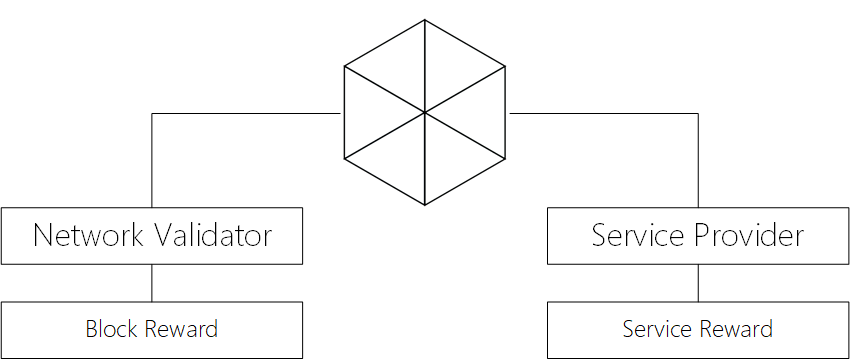
\includegraphics[width=4.0in]{img/staking.png}
    \caption{What Is Benefit For Our Token Holders}
    \label{fig:asure_architecture}
\end{figure}

\textbf{Network validators:}
Network validators need to stake a to be delivered amount of ASR tokens to validate transactions within the Asure network. In return the network validators receive the networks transaction fees in the form of ASR as an incentive for validating correct blocks. In case of fraudulent behaviour of a validator, the fraudulent validator will lose its stake to the network.

\textbf{Service providers:}
The ASR token serves as an incentive for service providers within the Asure platform to work correctly and as advertised within their SLA’s. Service providers must deposit ASR tokens which are retained in the event of non-compliance with the corresponding SLA. A service within the Asure network could be e.g. oracles, products, reinsurance and sales activity.\newline

Demand for ASR tokens will be created by the two following mechanisms: With the growth of the Asure network, blockchain or platform more Network Validators and Service Providers will need to stake ASR tokens. The more Network Validators and Service Providers want to earn, the more ASR tokens must be staked.\newline
The ASR token will be listed on crypto exchanges for public trading so that service providers of the Asure Network, blockchain or platform can buy and sell ASR tokens.
\newline\newline



\subsection{Token allocation}

It is very important that the community understands how Asures funds are going to be invested in the future in order to contribute to the idea of creating a world with an open decentralized autonomous system. See below how the investments will be allocated. 

\begin{itemize}
\item \textbf{Phase 1:} 20\% of all ASR tokens will be generated.
\item \textbf{Phase 2:} 80\% of all ASR tokens will be generated.
\end{itemize}

\subsubsection{Phase 1}

In the first phase 20\% of all ASR token will be distributed.

\begin{table}[H]
\begin{tabular}{llp{.62\textwidth}l}
  10\% & Public Pre-Sale & Contributions will be used to develop the network minimal viable product, and to build bigger community.\\
  5\% & Family \& Friends & Family and Friends receive their tokens as part of their compensation package.\\
  5\% & Bounty & Asure provides compensation for a number of tasks spread across marketing, bug reporting or even improving aspects of the Asure network, blockchain and platform.
\end{tabular}
\caption{\label{tab:table-name} Phase 1 - Token allocation}
\end{table}

\subsubsection{Phase 2}

In the second phase 80\% of all ASR tokens will be distributed.

\begin{table}[H]
\begin{tabular}{llp{.62\textwidth}l}
  35\% & Public Main-Sale & Contributions will be used to develop the platform, and to fund security, legal and operational needs. \\
  35\% & Foundation & Comprises foundation development and education initiatives, incentives to developers and to research blockchain, scaling, network, and platform.\\
  8\% & Team  & These are placed to acknowledge the time, effort and resources contributed to the Asure platform.  The Asure team receive their tokens as part of their compensation package, and team tokens will be vested.\\
  2\% & Advisors & Advisors receive their tokens as part of their compensation package.
\end{tabular}
\caption{\label{tab:table-name} Phase 2 - Token allocation}
\end{table}

\subsubsection{Vesting}
According to best practice and in order to protect investors and future participants of our platform, we will lock up our team’s tokens. The Asure Team will receive their tokens in twelve equal parts over two years.
The vesting ensures token course stability and commitment of all involved team members. If a holder attempts to transfer more ASR tokens than vested, the transaction will be blocked.
We are going to publish the smart contract to control vesting within our project. Hence, we will prove to the community our long-term commitment. 

\subsection{Funds allocation}

We envision that all ETH derived from the sale of Asure tokens will be allocated in the following manner:
\newline\newline

\begin{table}[H]
\begin{tabular}{llp{.6\textwidth}l}
  45\% & Platform R\&D & The creation of ongoing development of our Layer-2 network \\
  30\% & Marketing \& Operations & Additional staff and resources to cover day-to-day operations and prudent management as the organization expands. \\
  10\% & Legal & We are acutely aware of the need for rigorous compliance. We will need our own well-resourced legal support. Our principal concern is to fit within complex regulatory frameworks across the globe in order to make the growth of the community legally secure. \\
  10\% & Tax & Tax and organization development fees.\\
  5\% & Office Expenses & Office expenses and HR activities to build up
        a team to achieve roadmap goals
\end{tabular}
\caption{\label{tab:table-name}Funds allocation}
\end{table}

\subsection{KYC/AML}

The primary objective of token sale registration is to enforce a mandatory Know-Your-Customer (KYC) check to prevent identity theft, terrorist financing, Anti-money laundering (AML), and financial fraud. It also allows our team to understand our token holders better and manage risks appropriately.

The Asure tokens are not being offered or distributed to, as well as cannot be resold or otherwise alienated by their holders to citizens of, natural and legal persons, having their habitual residence, location or their seat of incorporation in the country or territory where transactions with digital coins are prohibited or in any manner restricted by applicable laws or regulations, or will become prohibited or restricted at any time after this agreement becomes effective (“Restricted Persons”).

We do not accept participation from the restricted persons and reserve the right to refuse or cancel the ASR token purchase requests at any time at our sole discretion when the information provided by the purchasers within the KYC procedure is not sufficient, inaccurate or misleading, or the purchaser is deemed to be a restricted person.

\subsection{Privacy and Security}
The security of your data is of great importance to us. There is no “cutting corners” when it comes to security, even under the pressure of running an ICO.  As such, please find below the measures which will be employed to ensure your privacy and security: 

All your data will be stored in an encrypted form on our servers
We don’t store your password as we only support external authentication providers like Google and Facebook
All the information required for the KYC process will be wiped out from our systems once the checks are completed

Asure will never share members’ personal data with 3rd parties without prior consent. In order to be on the safe side you should take these precautions: 

Never send any fiat money or crypto coins to any address during the registration process. There is only one public token sale date and it is specified on our 
website: https://www.asure.network
Bookmark the registration website, and never get to it following any email links.
Never trust emails related to the particular sale details (such as the information about soft or hard caps, Ethereum address to send to, etc.). Remember that sender’s email address can be easily forged. 
Never reply to our emails. Perform all your operations on our website only. You can check your registration status on our website using your account details. 


\subsection{Excluded participants}
Due to legal restrictions citizens and residents from the following countries are not eligible to acquire ASR tokens: American Samoa, Belarus, Burundi, Central African Republic, Cuba, Congo (Brazzaville), Congo (Kinshasa), Guam, Iraq, Iran, Lebanon, Libya, Northern Mariana Islands, North Korea, Puerto Rico, Somalia, Sudan, South Sudan, Syria, United States, US Virgin Islands, US Minor Outlying Islands, Venezuela, Yemen, Zimbabwe.
